\documentclass[12pt]{article}
\usepackage[utf8]{inputenc}
\usepackage[T2A]{fontenc}
\usepackage[english, russian]{babel}

\usepackage{color}
\usepackage{geometry}
\usepackage{indentfirst}
\usepackage{geometry}
\textheight = 24cm
\textwidth = 16cm
\oddsidemargin = 0cm
\topmargin = -1.5cm
\parindent = 24pt
\parskip = 0pt

\usepackage{graphicx}
\graphicspath{{images/}}
\usepackage[outdir=./images/]{epstopdf}

\usepackage{amsmath, amsthm, amssymb, thmtools}

\declaretheorem[style = definition, numbered = no, name = Определение]{definition}
\declaretheorem[style = plain, name = Лемма]{lemma}
\declaretheorem[style = plain, name = Теорема]{theorem}
\renewcommand{\qedsymbol}{\rule{0.6em}{0.6em}}
\DeclareFontFamily{OMX}{yhex}{}
\DeclareFontShape{OMX}{yhex}{m}{n}{<->yhcmex10}{}
\DeclareSymbolFont{yhlargesymbols}{OMX}{yhex}{m}{n}
\DeclareMathAccent{\wideparen}{\mathord}{yhlargesymbols}{"F3}

\usepackage{algorithmicx}
\usepackage[Algorithm, ruled]{algorithm}
\usepackage{algpseudocode}
\newcommand{\Break}{\State \textbf{break} }
\algnewcommand{\And}{\textbf{and}\xspace}

\usepackage{cite, enumerate}

\usepackage{authblk}
\title{$O(n)$-алгоритм слияния перекрывающихся триангуляций Делоне}
\author{Леонид Местецкий}
\author{Мария Готман}
\affil{ВМК МГУ}
\author{Наталья Дышкант}
\affil{НИВЦ}
\author{Елена Царик}
\affil{ТвГУ}
\date{}
\setcounter{Maxaffil}{0}
\renewcommand\Affilfont{\itshape\small}
\renewcommand\Authands{ и }

\begin{document}
\maketitle

\abstract{{\bf \color{red} ???}}

\section{Введение}
Задача построения триангуляции Делоне (ТД) $n$ сайтов-точек имеет нижнюю оценку вычислительной сложности  $O(n\log n)$.
В случаях, когда имеется некоторая дополнительная информация о структуре и связях сайтов, эта оценка может быть улучшена.
В частности, представляет интерес задача слияния двух триангуляций, когда исходное множество сайтов состоит из двух непересекающихся подмножеств $\bf{S} = \bf{S_1} \cup \bf{S_2}$, и триангуляции Делоне $Del(\bf{S_1})$ и $Del(\bf{S_2})$  исходных множеств $\bf{S_1}$ и $\bf{S_2}$ уже построены.
В \cite{Lee} описан алгоритм Ли-Шехтера слияния ТД за время $O(n)$ в случае, когда множества точек $\bf{S_1}$ и $\bf{S_2}$ линейно разделимы.
Мы рассматриваем более общую постановку задачи слияния ТД, когда множества сайтов $\bf{S_1}$ и $\bf{S_2}$ не пересекаются $\bf{S_1} \cap \bf{S_2} = \emptyset$, но перекрываются, т.е. пересекаются их выпуклые оболочки
$Conv(\bf{S_1})~\cap$ $Conv(\bf{S_2}) \ne \emptyset$.
Даны ТД $Del(\bf{S_1})$ и $Del(\bf{S_2})$, нужно построить ТД
$Del(\bf{S_1} \cup \bf{S_2})$ за время $O(n)$ в худшем случае.

В такой постановке задача слияния ТД до сих пор не рассматривалась, возможно, потому, что не представляла практического интереса.
Наш интерес к этой постановке связан с построением алгоритма для вычисления расстояния в метрическом пространстве функций двух переменных, заданных на конечных нерегулярных множествах точек.
Эта задача возникает, в частности, при анализе 3D поверхностей человеческих лиц, полученных в результате пространственного сканирования \cite{Dyshkant}.
Предложенная модель определяет расстояние между такими функциями на основе построения общей ТД.
При этом расстояние между моделями лиц определяется как минимальное по всем движениям множеств $\bf{S_1}$ и $\bf{S_2}$ на плоскости.
Таким образом, осуществляется подгонка пары поверхностей друг к другу.
И на каждой итерации подгонки выполняется слияние триангуляций.

Поскольку ТД и диаграмма Вороного (ДВ) $n$ сайтов являются двойственными графами и могут быть получены один из другого за время $O(n)$, для решения задачи в принципе можно использовать известные алгоритмы Киркпатрика \cite{Kirkpatrick} и Шазеля \cite{Chazelle}.
Алгоритм Киркпатрика \cite{Kirkpatrick} строит ДВ $Vor(\bf{S_1} \cup \bf{S_2})$ перекрывающихся множеств сайтов $\bf{S_1}$ и $\bf{S_2}$ на основе слияния ДВ $Vor(\bf{S_1})$ и $Vor(\bf{S_2})$. Для решения нашей задачи нужно преобразовать исходные ТД $Del(\bf{S_1})$, $Del(\bf{S_2})$ в $Vor(\bf{S_1})$, $Vor(\bf{S_2})$, построить $Vor(S_1 \cup S_2)$ с помощью алгоритма \cite{Kirkpatrick}, а затем преобразовать $Vor(\bf{S_1} \cup \bf{S_2})$ в $Del(\bf{S_1} \cup \bf{S_2})$.
Алгоритм Шазеля \cite{Chazelle} строит пересечение двух выпуклых многогранников в 3D-пространстве.
Для его использования применительно к нашей задаче требуется построить из исходных ТД $Del(\bf{S_1})$, $Del(\bf{S_2})$ сначала ДВ $Vor(\bf{S_1})$, $Vor(\bf{S_2})$, затем выпуклые многогранники. Затем нужно построить пересечение этих многогранников с помощью алгоритма \cite{Chazelle}. После этого из многогранника получается сначала ДВ $Vor(\bf{S_1} \cup \bf{S_2})$, а после $Del(\bf{S_1} \cup \bf{S_2})$.
Таким образом, используя алгоритм \cite{Kirkpatrick, Chazelle}, мы получаем решение за 3 и 5 шагов соответственно. И хотя вычислительная сложность этих решений остается $O(n)$, их практическая реализация весьма проблематична.
В отличие от этого, предлагаемый нами алгоритм находит $Del(\bf{S_1} \cup \bf{S_2})$ непосредственно на основе слияния исходных ТД $Del(\bf{S_1})$ и $Del(\bf{S_2})$.

Ещё одной причиной для прямого использования триангуляций Делоне служит то, что структура данных, описывающая ТД, обычно намного проще, чем структура ДВ.
В ТД все ребра одного типа, и имеют конечную длину.
Напротив, в ДВ существует специальный массив, хранящий бесконечные ребра диаграммы Вороного.
Наличие этого факта существенно осложняет задачу описания алгоритмов слияния.
Это и было одной из причин для разработки алгоритма Ли-Шехтера \cite{Lee}, хотя аналогичный алгоритм для ДВ, описанный в \cite{Shamos}, был уже известен.
Таким образом, актуальна задача описания и разработки эффективного алгоритма слияния пересекающихся триангуляций Делоне.

{\bf \color{red} Структура статьи следующая:}

\section{Терминология и постановка задачи}
Пусть на евклидовой плоскости задано $\bf{S}$ --- множество из
$n \ge 3$ точек, не все из которых лежат на одной прямой.
Эти точки будем называть {\it сайтами}.

{\it Триангуляцией} конечного множества точек $\bf{S}$ называется планарный граф с вершинами из $\bf{S}$,
все внутренние области которого являются треугольниками.
Триангуляция называется {\it выпуклой}, если минимальный многоугольник, охватывающий все ее треугольники, будет выпуклым.
Далее под термином {\it грань} будем понимать только конечную треугольную грань триангуляции.
Ребро и грань называются {\it инцидентными}, если они имеют две общие вершины.
Ребра, инцидентные одной грани, называются {\it смежными}.
Ребро, имеющее менее двух инцидентных граней, называется {\it открытым}.

Окружность называется {\it пустой}, если она не содержит внутри себя сайтов.
Прямая линия, по одну сторону от которой нет сайтов, называется {\it несобственной} пустой окружностью.
Окружность, проходящая через сайт, называется {\it инцидентной} этому сайту.
{\it Ребром Делоне} называется ребро, инцидентные сайты которого имеют общую пустую инцидентную окружность.
{\it Гранью Делоне} называют грань, вершины которой имеют общую пустую инцидентную окружность.

Дадим два эквивалентных определения:

\begin{definition}
{\it Триангуляцией Делоне (ТД) $Del(\bf{S})$} множества точек $\bf{S}$ называется выпуклая триангуляция,
у которой описанная окружность каждой треугольной грани является пустой,
т.е. все грани которой являются гранями Делоне.
\end{definition}

\begin{definition}
{\it Триангуляцией Делоне} множества точек $\bf{S}$ называется выпуклая триангуляция,
у которой для каждого ребра существует пустая инцидентная сайтам-вершинам окружность,
т.е. все ребра которой являются ребрами Делоне.
\end{definition}

{\it Пучком} сайта $p \in \bf{S}$ называют множество ребер триангуляции, инцидентных сайту $p$.
Пучок сайтов будем представлять в виде двунаправленного циклического списка сайтов $p_1, \ldots, p_k$,
смежных с $p$ в триангуляции, так чтобы они шли в направлении обхода против часовой стрелки относительно $p$.

Задача слияния двух перекрывающихся триангуляций Делоне ставится следующим образом.
Даны два конечных линейно неразделимых множества сайтов $\bf{B}$ и $\bf{W}$ (считаем, что сайты раскрашены в два цвета: множество черных сайтов $\bf{B}$ и множество белых сайтов $\bf{W}$),
а также их триангуляции Делоне $Del(\bf{B})$ и $Del(\bf{W})$.
Нужно построить триангуляцию Делоне на объединенном множестве сайтов $Del(\bf{B} \cup \bf{W})$.

Пример исходных данных и искомой триангуляции приведен на рис. \ref{fig:model_data}.

\begin{figure}[htb!]
	\begin{minipage}[h]{0.49\linewidth}
		\center{\includegraphics[width=1\linewidth]{model_data.png}}
	\end{minipage}
	\hfill
	\begin{minipage}[h]{0.49\linewidth}
		\center{\includegraphics[width=1\linewidth]{model_res.png}}
	\end{minipage}
	\caption{Исходные триангуляции и объединенная триангуляция}
	\label{fig:model_data}
\end{figure}

\section{\color{red} Problem discussion and related work}

\section{Структура алгоритма}
В объединенной триангуляции Делоне $Del(\bf{B} \cup \bf{W})$ существуют ребра двух типов:
одноцветные, которые были взяты из исходных триангуляций, и разноцветные, сайты-вершины которых взяты из разных исходных триангуляций.

В объединенной триангуляции существуют максимальные связные одноцветные подмножества вершин и ребер,
переходящие без изменений из исходных триангуляций, которые будем называть {\it лоскутами}.
Ребра и грани, не вошедшие в лоскуты при слиянии триангуляций, должны быть разрушены.
Такие связные подмножества будем называть {\it разрезами}.
При построении разрезов будут удалены некоторые грани, что приведет к образованию открытых ребер.
При объединении будут образовываться новые разноцветные ребра, называемые {\it стежками}.
Максимальные связные подмножества разноцветных ребер и граней объединенной триангуляции будем называть {\it швами}.

При данных определениях построение объединенной триангуляции Делоне состоит из нескольких частей: построения разрезов,
выделения лоскутов исходных триангуляций и построения швов.

{\it Стартером} будем называть пару разноцветных сайтов, образующих ребро Делоне,
еще не включенное в объединенную триангуляцию.
Процесс нахождения стартера будет подробнее описан ниже.
Стартер нужен для запуска процесса построения разрезов и швов.
На рис. \ref{pic:dir} черная жирная линия обозначает стартер, жирная пунктирная новый стежок, построенный в направлении перед стартером.

\begin{figure}[htb!]
	\begin{minipage}[h]{0.49\linewidth}
		\center{\includegraphics[width=0.7\linewidth]{starter.png}}
	\end{minipage}
	\hfill
	\begin{minipage}[h]{0.49\linewidth}
		\center{\includegraphics[width=0.7\linewidth]{direct_starter.png}}
	\end{minipage}
	\caption{Построение новых стежков}
	\label{pic:dir}
\end{figure}

Шов может быть двух типов.
{\it Разомкнутым} швом называется шов, имеющий два стежка, принадлежащих выпуклой оболочке объединенной триангуляции,
то есть принадлежащих граничным ребрам $Del(\textbf{B} \cup \textbf{W})$.
{\it Циклическим} называется шов, имеющий только внутренние ребра объединенной триангуляции.

В процессе построения разомкнутого шва сначала находим одну его часть,
затем продолжаем движение по другую сторону стартера и находим оставшуюся часть разреза.
В циклическом шве в некоторый момент времени стартер совпадет с новым стежком,
на этом построение шва будет закончено.

Введем понятие минимального остовного дерева.
{\it Минимальным остовным деревом (МОД)} триангуляции Делоне называется ее связный подграф,
имеющий наименьшую суммарную длину ребер.
Пусть на плоскости задано $N$ точек.
{\it Евклидовым МОД (ЕМОД)} называется связный подграф,
вершинами которого являются все $N$ точек, суммарная длина всех ребер которого минимальна.
Известно, что МОД ТД является ЕМОД для множества сайтов ТД \cite[стр. 227, 277]{Preparata}.
МОД исходных триангуляций Делоне понадобятся в процессе построения стартеров.

{\bf Общая схема слияния перекрывающихся триангуляций Делоне:}

\begin{enumerate}
	\item Поиск начального стартера
	\item \label{alg_ru:seam} Построение разреза и шва от найденного стартера
	\item Поиск очередного стартера
	\item Если стартер найден, перейти к пункту \ref{alg_ru:seam}, иначе закончить работу алгоритма
\end{enumerate}

\section{Описание алгоритма}
Пусть множество $\textbf{B}$ содержит $n_1$ точек c координатами
$(x_{11}, y_{11}), (x_{12}, y_{12}), \ldots, (x_{1n_1}, y_{1n_1})$,
множество $\textbf{W}$ --- $n_2$ точек с координатами
$(x_{21}, y_{21}), (x_{22}, y_{22}), \ldots, (x_{2n_2}, y_{2n_2})$.
На вход алгоритму подаются координаты первого и второго множества точек исходных триангуляций:
\begin{equation}\label{eq:points01}
\begin{split}
	pointsB = \{(x_{11}, y_{11}), (x_{12}, y_{12}), \ldots, (x_{1n_1}, y_{1n_1}) \} \\
	pointsW = \{(x_{21}, y_{21}), (x_{22}, y_{22}), \ldots, (x_{2n_2}, y_{2n_2}) \}
\end{split}
\end{equation}

Объединенное множество точек $\textbf{B} \cup \textbf{W}$,
содержащее $n = n_1 + n_2$ точек, будем обозначать:
\begin{equation}\label{eq:points2}
	points = pointsB + pointsW\
\end{equation}

На вход также подается структура данных, содержащая информацию о ребрах и/или гранях исходных триангуляций.
Выбор структуры данных сильно влияет на дальнейшую сложность вычислений.
Поэтому, рассмотрим более подробно этот пункт.

\subsection{Выбор структуры данных}
В нашей задаче будут часто производиться коррекции пучков сайтов,
поэтому операцию добавления и удаления ребер из пучка нужно производить очень эффективно.
Из предложенных в \cite[стр. 11-17]{Skvortsov} для нашей задачи лучше всего подходит структура данных {\itshape <<Узлы с соседями>>} (рис.\ref{pic:struct}).
Такая структура для каждого сайта хранит его координаты на плоскости и список номеров смежных сайтов в обходе против часовой стрелки.
Рассматриваемая структура данных неявно содержит ребра триангуляции, грани в данной структуре не хранятся вообще,
что в нашей задаче, вообще говоря, и не нужно.

\begin{figure}[htb!]
	\center{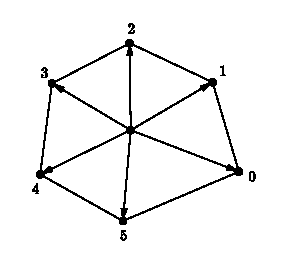
\includegraphics[width=0.4\linewidth]{struct.eps}}
	\caption{Структура данных {\itshape <<Узлы с соседями>>}}
	\label{pic:struct}
\end{figure}

Для хранения описанной выше информации для каждого сайта создается двунаправленный список номеров смежных сайтов
в порядке обхода против часовой стрелки
в соответствии с их номером в объединенном множестве точек (\ref{eq:points2}):

\begin{equation}\label{eq:neib}
\begin{split}
	neighbors = \{list_1, list_2, \ldots, list_n\},
\end{split}
\end{equation}
где $list_i$ --- список смежных сайтов в порядке обхода против часовой стрелки для $i$-ого сайта.

Пусть сайт $A$ предшествует сайту $B$ в пучке сайта $C$, тогда верно:
\begin{equation}\label{eq:op}
\begin{split}
	A = neighbors[C].prev(B) \\
	B = neighbors[C].next(A)
\end{split}
\end{equation}

\subsection{Построение разрезов и швов триангуляций Делоне}
Процесс построения разрезов и швов основан на проверке условия Делоне для ребер триангуляции,
которую можно осуществлять при помощи углового критерия:

\begin{lemma}
\label{th:lem1}
Пусть $\textbf{S}$ --- множество сайтов, для пары $A, B \in \textbf{S}$ выполнено условие Делоне $\Leftrightarrow$
для любых других двух сайтов $C, D \in \textbf{S}$, лежащих по разные стороны от $AB$, справедливо:
$\angle ACB + \angle ADB \le 180^\circ$ и $\angle ABD \ge \angle ACD$
\end{lemma}

\begin{proof}
Докажем, что $\angle ACB + \angle ADB \le 180^\circ$.
Рассмотрим окружность, инцидентную сайтам $A$ и $B$ (рис.\ref{pic:lem1} левый).
Пусть $E$ --- середина $AB$.
Отрезки $EC$ и $ED$ пересекают окружность в точках $C'$ и $D'$ соответственно.
В четырехугольнике $AC'BD'$, вписанном в окружность, имеем $\angle AC'B+\angle AD'B = 180^\circ$.
Если окружность пустая, то $\angle ACB \le \angle AC'B$ и $\angle ADB \le \angle AD'B$.
Тогда получаем: $\angle ACB + \angle ADB \le \angle AC'B + \angle AD'B = 180^\circ$.
И наоборот, если $\angle ACB + \angle ADB > 180^\circ$, то пустой окружности, инцидентной $A$ и $B$, не существует, что и доказывает утверждение.

Докажем второе утверждение.
Предположим противное, пусть $\angle ABD < \angle ACD$.
Построим описанную окружность для треугольника $\triangle ABD$ (рис.\ref{pic:lem1} правый).
Тогда $C$ лежит внутри нее.
Пусть $C'$ --- точка пересечения прямой $CD$ с окружностью.
В четырехугольнике $AC'BD$, вписанном в окружность, имеем $\angle AC'B + \angle ADB = 180^\circ$.
Поскольку $\angle AC'B < \angle ACB$, получаем, что $\angle ACB + \angle ADB > 180^\circ$.
А тогда для $AB$ согласно первому утверждению леммы не выполняется условие Делоне.
Значит, предположение $\angle ABD < \angle ACD$ неверно, и утверждение леммы выполняется.
\end{proof}

\begin{figure}[htb!]
	\begin{minipage}[h]{0.49\linewidth}
		\center{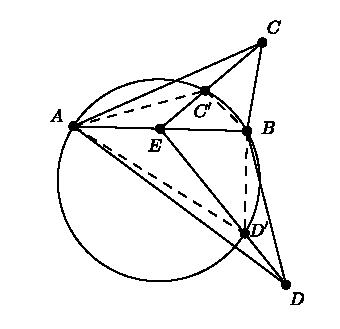
\includegraphics[width=0.7\linewidth]{lem1a.eps}}
	\end{minipage}
	\hfill
	\begin{minipage}[h]{0.49\linewidth}
		\center{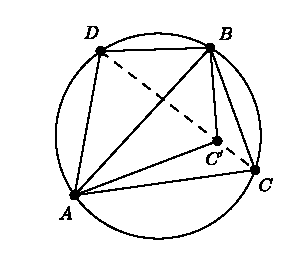
\includegraphics[width=0.7\linewidth]{lem1b.eps}}
	\end{minipage}
	\caption{Пояснение к лемме \ref{th:lem1}}
	\label{pic:lem1}
\end{figure}

Пусть найдена разноцветная пара сайтов $A$ и $B$, такая что ребро $AB$ образует ребро Делоне в объединенной триангуляции,
ещё не включенное в нее.
Например, $AB$ является стартером.
Присоединение ребра $AB$ к пучкам сайтов-вершин $A$ и $B$ может привести к нарушению условия Делоне для некоторых ребер из этих пучков.
Все ребра, не удовлетворяющие условию Делоне, должны быть разрушены на этом этапе.
Рассмотрим, подробнее этот процесс.

\begin{figure}[htb!]
	\begin{minipage}[h]{0.49\linewidth}
		\center{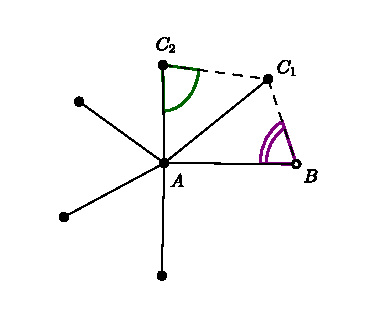
\includegraphics[width=0.9\linewidth]{deleteWrongEdges1.eps}}
	\end{minipage}
	\hfill
	\begin{minipage}[h]{0.49\linewidth}
		\center{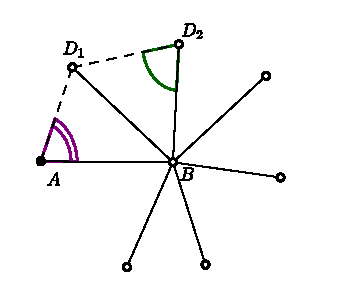
\includegraphics[width=0.9\linewidth]{deleteWrongEdges2.eps}}
	\end{minipage}
	\caption{Коррекция одноцветных ребер}
	\label{pic:deleteWrongEdges}
\end{figure}

Пусть $AC_1$ и $AC_2$ одноцветные ребра пучка $A$,
что сайты $B$, $C_1$ и $C_2$ идут в порядке обхода против часовой стрелки в пучке сайта $A$ (рис. \ref{pic:deleteWrongEdges} левый).
Для ребра $AC_1$ нарушено условие Делоне, если $\angle AC_2C_1 + \angle ABC_1 > 180^\circ$.
В этом случае ребро $AC_1$ удаляется из объединенной триангуляции, а ребро $AC_2$ подвергается аналогичной проверке.
Если же для ребра $AC_1$ условие Делоне выполнено, то ребро $AC_1$ сохраняется в объединенной триангуляции,
проверка условия Делоне для остальных ребер не производится.

Аналогичным образом выполняется коррекция пучка сайта $B$ в направлении обхода по часовой стрелке (рис. \ref{pic:deleteWrongEdges} правый).

После этого ребро $AB$ разворачивается, и снова производятся действия по коррекции ребер.
Таким образом, пучки сайтов $A$ и $B$ будут скорректированы как по часовой стрелке, так и против нее.
На этом вставка нового ребра $AB$ заканчивается.

Во время выполнения алгоритма часть ребер будет удалена.
Все удаленные ребра занесем в отдельный список $deleteEdges$, эта информация понадобится нам при поиске последующих стартеров.
Об этом подробно будет рассказано ниже.

Приведем формальное описание процедуры коррекции пучков сайтов (алгоритм \ref{alg:deleteWrongEdges}),
параметрами являются номера сайтов $A$ и $B$, для которых проводится коррекция, $reverse$ является необязательным параметром, нужен, чтобы развернуть ребро $AB$ и продолжить коррекцию ребра $BA$.

\begin{algorithm}[htb!]
\floatname{algorithm}{Алгоритм}
\begin{algorithmic}[1]
\Procedure{deleteWrongeEdges$(a, b, reverse = 0)$}{}
	\State $c_1 := neighbors[a].prev(b)$ \Comment{Обрабатываем пучок сайта $A$}
	\State $c_2 := neighbors[a].prev(c_1)$
	\While{$\angle abc_1 + \angle ac_2c_1 > 180^\circ$}
	    \State $deleteEdges.add(ac_1)$
		\State Удалить ребро $ac_1$ из ТД
		\State $c_1 := c_2$
		\State $c_2 := neighbors[a].prev(c_2)$
	\EndWhile
    	\State $d_1 := neighbors[b].next(a)$ \Comment{Обрабатываем пучок сайта $B$}
	\State $d_2 := neighbors[b].next(d_1)$
	\While{$\angle bad_1 + \angle bd_2d_1 > 180^\circ$}
		\State $deleteEdges.add(bd_1)$
		\State Удалить ребро $bd_1$
		\State $d_1 := d_2$
		\State $d_2 := neighbors[b].next(d_2)$
	\EndWhile
	\If{$reverse == 0$} \Comment{Развернуть ребро $AB$, продолжить проверку}
		\State deleteWrongeEdges$(b, a, 1)$
	\EndIf
\EndProcedure
\end{algorithmic}
\caption{Коррекция пучков сайтов}
\label{alg:deleteWrongEdges}
\end{algorithm}

Пучки, для которых выполнена описанная коррекция, будем называть {\itshape правильными}.
Рассмотрим процесс образования новых разноцветных ребер объединенной триангуляции Делоне:

\begin{lemma}
\label{th:lem2}
Пусть пучки сайтов $A$ и $B$ разноцветного ребра $AB$ являются правильными.
Точка $C$ следует за точкой $B$ в пучке сайта $A$, точка $D$ предшествует точке $A$ в пучке сайта $B$,
тогда если $\angle ACB > \angle ADB$, то $CB$ является новым ребром Делоне, иначе $AD$ является новым ребром Делоне.
\end{lemma}

\begin{proof}
Поскольку $AB$ ребро Делоне, то существует пустая окружность, инцидентная сайтам $A$ и $B$ (рис.\ref{pic:lem2}).
Значит, сайты $C$ и $D$ лежат вне этой окружности.
Рассмотрим описанные окружности треугольников $\triangle ACB$ и $\triangle ADB$.
Очевидно, что дуги этих окружностей, лежащие ниже $AB$, целиком попадают внутрь пустой окружности ребра Делоне, следовательно, снизу от $AB$ внутри этих окружностей не может оказаться какой-либо сайт.
А выше ребра $AB$ одна из этих окружностей также является пустой, причем та, у которой угол треугольника, лежащий против стороны $AB$, больше
(если углы $\angle ACB$ и $\angle ADB$ равно, то можно выбрать любое ребро).
Это вытекает из правильности пучков сайтов $A$ и $B$.
\end{proof}

\begin{figure}[htb!]
	\center{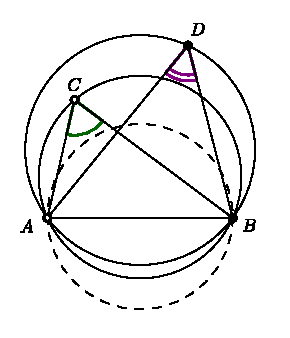
\includegraphics[width=0.3\linewidth]{lem2.eps}}
	\caption{Пояснение к лемме \ref{th:lem2}}
	\label{pic:lem2}
\end{figure}

Лемма \ref{th:lem2} описывает процесс образования новых разноцветных стежков при построении шва.
Из начального стежка $AB$ получаем следующий стежок $AD$ (или $BC$).
Далее возвращаемся к предыдущему шагу, производим коррекции пучков сайтов $A$ и $D$ (или $B$ и $C$ соответственно),
пока очередной стежок не окажется ребром выпуклой оболочки или шов не окажется циклическим.
Если очередной стежок оказался ребром выпуклой оболочки, то нужно развернуть стартер, и продолжить построение шва с другой стороны от него.

Таким образом, если найдено разноцветное ребро, удовлетворяющее условию Делоне,
то процесс построения разреза и шва можно проделывать рассмотренным способом.
Процедура, описывающая этот процесс, представлена в алгоритме \ref{alg:sewTriangle}.
На вход подаются номера точек $a$ и $b$, являющихся стартером.

\begin{algorithm}[htb!]
\floatname{algorithm}{Алгоритм}
\begin{algorithmic}[1]
\Procedure{sewTriangle$(a_0, b_0, reverse = 0)$}{}
    \State $[a, b] := [a_0, b_0]$
	\While{True}
		\State $deleteWrongEdges(a, b)$
		\State $c := neighbors[a].prev(b)$
		\State $d := neighbors[b].next(a)$
		\If{$\angle acb \ge \angle adb~\And~\angle acb < \pi$} \Comment{$cb$ --- новое ребро}
			\State Добавить ребро $cb$ в триангуляцию 
			\If{$[c, b] \neq [a_0, b_0]$}
				\State $a := c$
			\Else
				\State $reverse := 1$ \Comment{Шов является циклическим}
				\Break
			\EndIf
		\ElsIf{$\angle adb > \angle acb~\And~\angle adb < \pi$} \Comment{$ad$ --- новое ребро}
			\State Аналогично ребру $cb$
		\Else
			\Break
		\EndIf
	\EndWhile
	\If{$reverse == 0$} \Comment{Построение шва с другой стороны от стартера}
		\State sewTriangle$(a_0, b_0, 1)$
	\EndIf
\EndProcedure
\end{algorithmic}
\caption{Построение разреза и шва триангуляции}
\label{alg:sewTriangle}
\end{algorithm}

\subsection{Поиск стартеров}
В задаче поиска первого и последующих стартеров используется различная информация о триангуляциях.
Первый стартер ищется на основе начальной информации,
в процессе поиска последующих используется информация о уже построенных швах и разрушенных при этом одноцветных ребрах, хранящихся в $deleteEdges$.

Рассмотрим условия существования стартеров (разноцветных ребер Делоне).

\begin{lemma}
\label{th:lem3}
Сайт имеет инцидентное разноцветное ребро Делоне $\Leftrightarrow$ существует инцидентная ему окружность, внутри которой нет сайтов одного с ним цвета, но есть сайты противоположного цвета на ней или внутри нее.
\end{lemma}

\begin{proof}
Достаточность. Пусть для некоторого сайта $A$ существует инцидентная ему окружность с центром $C$,
внутри которой нет ни одного сайта того же цвета, что и $A$,
но есть сайты противоположного цвета $D_1, D_2, \ldots, D_k, k \ge 1$ другого цвета внутри или на окружности (рис. \ref{pic:lem3}).
Рассмотрим множество окружностей, инцидентных парам сайтов $A$ и $D_i, i = 1, \ldots, k$,
имеющих в точке $A$ общую касательную с окружностью с центром в точке $C$.
Окружность, имеющая минимальный радиус, является пустой, и она инцидентна разноцветной паре сайтов.
Значит, эта пара сайтов образует ребро Делоне и может являться стартером.

Необходимость. Есть пара сайтов, образующая ребро Делоне с инцидентной пустой окружностью.
Эта окружность и будет удовлетворять условию леммы.
\end{proof}

\begin{figure}[htb!]
	\center{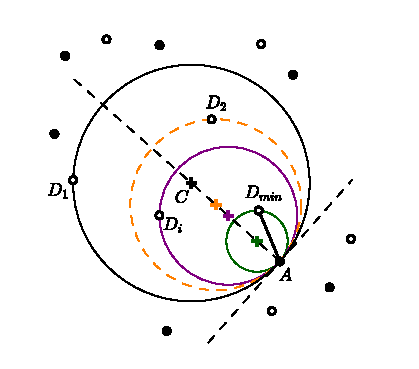
\includegraphics[width=0.4\linewidth]{lem3.eps}}
	\caption{Условие существования стартера}
	\label{pic:lem3}
\end{figure}

Согласно лемме \ref{th:lem3}, если существует сайт $A$ и инцидентная ему окружность $O$, удовлетворяющая условию леммы,
то поиск стартера сводится к перебору сайтов $D_1, D_2, \ldots, D_k$, $k \ge 1$, отличного от $A$ цвета,
внутри этой окружности и выбору сайта $D_{min}$,
такого что инцидентная $A$ и $D_{min}$ окружность имеет с окружностью $O$ общую касательную в точке $A$ и
минимальный радиус из всех таких окружностей, инцидентных $A$ и $D_i$.
Тогда ребро $AD_{min}$ можно использовать в качестве стартера.

\subsubsection{Поиск первого стартера}
Будем говорить, что сайт $A$ {\itshape лежит левее} сайта $B$,
если $A$ предшествует $B$ при лексикографическом упорядочивании сайтов по возрастанию координат $(x, y)$.

\begin{figure}[htb!]
	\center{\includegraphics[width=0.6\linewidth]{starterExample.png}}
	\caption{Поиск первого стартера}
	\label{pic:starterExample}
\end{figure}

Пусть $\textbf{B}$ и $\textbf{W}$ множества сайтов исходных триангуляций.
Найдем сайты $B_{min}$ и $W_{min}$, являющиеся самыми левыми в соответствующем множестве точек $\textbf{B}$ и $\textbf{W}$.
Не ограничивая общности, будем считать, что $B_{min}$ лежит левее, чем $W_{min}$  (рис. \ref{pic:starterExample}).
Рассмотрим окружность $O$, инцидентную сайтам $B_{min}$ и $W_{min}$ с центром на луче, параллельном оси $Ox$,
выходящим из точки $W_{min}$ влево.
Окружность $O$ не содержит ни одного сайта из $\textbf{W}$, потому что лежит левее самого левого сайта этого множества $W_{min}$,
и содержит сайт $B_{min}$ на границе окружности.
Внутри этой окружности может не оказаться ни одного сайта, тогда пара $W_{min}$ и $B_{min}$ образует стартер.
Если же она не пустая, то часть сайтов из $\textbf{B}$ попадет внутрь этой окружности.
Тогда точка $W_{min}$ и окружность $O$ удовлетворяют условиям леммы \ref{th:lem3}.
То есть первый стартер найден.
Алгоритм \ref{alg:findFirstStarter} описывает поиск первого стартера.

\begin{algorithm}[htb!]
\floatname{algorithm}{Алгоритм}
\begin{algorithmic}[1]
\Procedure{findFirstStarter()}{}
	\State $b_{min}$ --- самая левая точка множества $pointsB$ 
	\State $w_{min}$ --- самая левая точка множества $pointsW$
	\State $starter_0 := w_{min}$ \Comment{Не ограничивая общности, $b_{min}$ лежит левее $w_{min}$}
	\State $R_{min} := Inf$
	\For{$p \in pointsB$}
		\State $r$ --- радиус окружности с центром на горизонтальном луче из точки $w_{min}$ влево,
		инцидентной сайтам $p$ и $w_{min}$
		\If{$r < R_{min}$}
			\State $R_{min} := r$
			\State $starter_1 := p$ \Comment{Объявить $p$ концом стартера}
		\EndIf
	\EndFor
	\State \Return $[starter_0, starter_1]$
\EndProcedure
\end{algorithmic}
\caption{Поиск первого стартера}
\label{alg:findFirstStarter}
\end{algorithm}

Время поиска первого стартера складывается из вычисления самых левых точек множеств $\textbf{B}$ и $\textbf{W}$ и
перебора точек из множества $\textbf{B}$ (или $\textbf{W}$) по методу из леммы \ref{th:lem3},
то есть линейно по общему числу сайтов, и равно $O(n_1 + n_2)$.

\subsubsection{Минимальные остовные деревья}
Задача поиска последующих стартеров основана на использовании минимальных остовных деревьев (МОД) исходных триангуляций Делоне.
МОД исходных триангуляций вычисляются один раз, поэтому это действие можно отнести к этапу предобработки, предшествующем непосредственному слиянию исходных триангуляций.
Теоретическая оценка трудоемкости задачи построения минимального остова составляет $O(n\log n)$.
Поскольку известно, что МОД является подграфом триангуляции Делоне, и на ее основе МОД может быть построен за линейное время (рис. \ref{pic:mst}).
Такой вычислительной сложностью обладает алгоритм Черитона-Тарьяна \cite[стр. 226-230]{Preparata}.

\begin{figure}[htb!]
	\center{\includegraphics[width=0.4\linewidth]{mst.png}}
	\caption{Евклидово минимальное остовное дерево триангуляции Делоне}
	\label{pic:mst}
\end{figure}

Поиск последующих стартеров основан на том, что при построении разреза в триангуляции Делоне нарушается ее связность,
поэтому среди разрушенных ребер обязательно окажется ребро МОД этой триангуляции Делоне.

Будем называть окружность, диаметром которой является ребро МОД, {\itshape окружностью влияния ребра}.
Леммы \ref{th:lem4} и \ref{th:lem5} описывают свойства минимальных остовных деревьев,
которые понадобятся для теоретической оценки сложности алгоритма.

\begin{lemma}
\label{th:lem4}
Окружность влияния ребра МОД является пустой окружностью ТД.
\end{lemma}

\begin{proof}
Предположим противное: пусть $AB$ –-- ребро МОД и внутрь окружности с диаметром $AB$ попадает точка $C$.
В $\triangle ABC$ угол $\angle C$ тупой, поэтому $|AC| < |AB|$ и $|BC| < |AB|$. Тогда если ребро $AB$ исключить из МОД, то дерево распадется на две связные компоненты, в одной из которых находится вершина $C$.
Если $C$ оказалась в одной компоненте с $A$, то включаем в дерево ребро $CB$, которое короче $AB$.
Аналогично, если $C$ находится в одной компоненте с $B$, меняем ребро $AB$ на $AC$.
В обоих случаях получаем дерево с длиной ребер меньшей, чем у исходного, что противоречит принадлежности $AB$ к МОД. 
\end{proof}

\begin{lemma}
\label{th:lem5}
Расстояние между центрами двух ребер МОД не меньше, чем половина длины каждого ребра.
\end{lemma}

\begin{proof}
Предположим противное. Пусть $AA_1$ и $BB_1$ –-- ребра МОД с серединами $A_0$ и $B_0$ такие, что $|A_0B_0 \le AA_0$ (рис.\ref{pic:lem5}).
Тогда их окружности влияния пересекаются в некоторых точках $C$ и $D$.
Не нарушая общности, предположим, что $AB \ge A_1B_1$.
Из точки $C$ проведем диаметры $CE$ и $CF$ кругов $A_0$ и $B_0$ соответственно.
В $\triangle CDE$ угол $\angle CDE$ прямой, а в $\triangle CDF$ угол $\angle CDF$ тоже прямой, следовательно, $EF$ проходит через точку $D$.

Из леммы \ref{th:lem4} следует, что точка $A$ лежит на дуге $ED$, а точка $B$ – на дуге $DF$.
Углы $\angle EAD$ и $\angle DBF$ тупые, поскольку дуги $ED$ и $DF$ меньше полуокружностей.
Следовательно, $AB < AD + DB < ED + DF = EF = 2A_0B_0$, т.е. $AB < AA_1$.
Поскольку $A_1B_1 \le AB$, то и $A_1B_1 < AA_1$.
Покажем, что в этом случае $AA_1$ не может быть ребром МОД.
Действительно, если удалить из покрывающего дерева ребро $AA_1$, то одна из точек $A$ или $A_1$ окажется в одной компоненте с ребром $BB_1$.
Если это точка $A$, то заменяем $AA_1$ на $A_1B_1$ и получаем покрывающее дерево с меньшей длиной ребер.
Если это точка $A_1$, то заменяем $AA_1$ на $AB$ с тем же результатом.
Полученное противоречие доказывает утверждение леммы. 

\end{proof}

\begin{figure}[htb!]
	\center{\includegraphics[width=0.35\linewidth]{lem5.png}}
	\caption{Пояснение к лемме \ref{th:lem5}}
	\label{pic:lem5}
\end{figure}

Идея использования МОД для поиска стартеров основана на том очевидном факте, что если при образовании разреза в ТД нарушается ее связность, то обязательно среди разрушенных ребер окажется ребро МОД этой ТД.

\subsubsection{Поиск последующих стартеров}
{\itshape Мостами} будем называть ребра исходных триангуляций,
входящие в МОД, разрушенные при построении очередного разреза (при выполнении функции $deleteWrongeEdges$).
При построении разрезов удалялись ребра $AC_1$ и $BD_1$, переставшие удовлетворять лемме \ref{th:lem1},
при этом сайты $A$ и $B$ будем называть {\it закрепленными}, потому что они имеют разноцветные инцидентные ребра, а значит, они прикреплены к объединенной триангуляции, а $C_1$ и $D_1$ будем называть {\it свободными}.
Свободные сайты могут быть присоединены к объединенной триангуляции только при помощи построения новых швов,
поэтому существование свободного сайта говорит о том, что построение объединенной триангуляции ещё не завершено:

\begin{lemma}
\label{th:lem6}
Существует стартер, инцидентный свободному сайту.
\end{lemma}

\begin{proof}
Рассмотрим мост, инцидентный свободному сайту.
По определению он является ребром МОД одной из исходных триангуляций и тогда, согласно лемме \ref{th:lem4}, внутри его окружности влияния нет сайтов одного с ним цвета. Но поскольку это ребро было разрушено при построении разреза, это означает, что внутрь этой окружности попали сайты противоположного цвета. Следовательно, для свободного сайта выполнено условие леммы \ref{th:lem3}, что и доказывает утверждение.
\end{proof}

Пусть сайты $A$ и $B$ --- разноцветные, сайт $A$ входит в триангуляцию Делоне $T$.
{\itshape Максимальными пустыми окружностями} будем называть пустые окружности,
которые не содержатся внутри других пустых окружностей, не совпадающих с ними.
Рассмотрим множество окружностей, инцидентных $A$ и являющихся пустыми относительно сайтов триангуляции $T$.
В этом множестве существуют максимальные пустые окружности, которые являются описанными окружностями граней триангуляции $T$,
инцидентные сайту $A$. 
В случае, когда $A$ принадлежит границе выпуклой оболочки триангуляции Делоне $T$,
несобственные окружности также будут максимальными пустыми окружностями, инцидентными сайту $A$.

\begin{lemma}
\label{th:lem7}
Пусть $AB$ --- стартер. Тогда сайт $B$ попадает внутрь хотя бы одной из максимальных пустых окружностей в $T$, инцидентных сайту $A$.
\end{lemma}

\begin{proof}
Любая пустая окружность, инцидентная сайту $A$, принадлежит объединению максимальных пустых окружностей сайта $A$.
Поэтому если сайты $A$ и $B$ образуют ребро Делоне, то инцидентная им пустая окружность лежит также в этом объединении.
\end{proof}

\begin{figure}[htb!]
	\center{\includegraphics[width=0.6\linewidth]{nextStarter.png}}
	\caption{Поиск последующих стартеров}
	\label{pic:nextStarter}
\end{figure}

Пусть $AB$ --- мост, сайт $A$ является закрепленным, сайт $B$ --- свободным (рис. \ref{pic:nextStarter}).
Сайты $A$ и $B$ имеют один и тот же цвет (на рисунке – черный) и в окружности влияния моста находятся лишь сайты противоположного цвета.
Согласно лемме \ref{th:lem6} свободный сайт $B$ может быть выбран в качестве первого сайта стартера.
Сайт $B$ попадает внутрь максимальных пустых окружностей триангуляции белых сайтов.
На рисунке это описанные окружности треугольных граней $\triangle C_3C_4C_5,~\triangle C_3C_5C_6,~\triangle C_6C_5C_7$.
Согласно лемме \ref{th:lem7} для нахождения второго сайта стартера можно выполнять перебор не по всем вершинам,
а только по вершинам граней, внутри описанных окружностей которых лежит сайт $B$.
Таким образом, поиск второго сайта осуществляется среди вершин этих граней,
причем только тех из них, которые попадают внутрь окружности влияния моста,
в нашем примере среди сайтов $C_3, C_4$ и $C_6$.

Сайт $A$ уже включен в объединенную триангуляцию,
поэтому можно оценить положение свободного сайта $B$ относительно этой триангуляции.
Задачу определения местоположения свободного сайта относительно триангуляции,
в которую уже включен закрепленный сайт, будем называть {\itshape локализацией моста}.
Для этого найдем точки $C_1$ и $C_2$ (рис.\ref{pic:nextStarter}, такие, что $AB$ находится между $AC_1$ и $AC_2$, а угол $\angle AC_1C_2$ минимален.
При этом ребро $C_1C_2$ пересекает мост $AB$.
Для определенности будем считать, что сайт $C_1$ находится слева от $AB$, $C_2$ --- справа.
Точка $C_3$ является следующей в направлении по часовой стрелке после $C_2$ в пучке $C_1$ и предыдущей в направлении обхода против часовой стрелки после $C_1$ в пучке $C_2$, то есть $C_3 = neighbours[C_1].next(C_2) = neighbours[C_2].prev(C_1)$.
Из ребер $C_1C_3$ и $C_2C_3$ выбираем то, которое пересекает $AB$, и продолжаем трассировку.
Если ни одно из этих ребер не пересекает $AB$, значит, локализация сайта $B$ закончена,
мы имеем либо грань, в которой лежит точка $B$, либо ребро, определяющее полуплоскость, в которой лежит $B$.

Найденная грань имеет описанную окружность, которая содержит свободный сайт $B$, но эта окружность может быть не минимального радиуса.
Для поиска окружности минимального радиуса с центром на мосту $AB$, проходящей через точку $B$,
переберем точки, лежащие в пучках вершин грани (полуплоскости), являющейся решением задачи локализации моста.
То есть последовательно будем строить окружность по двум точкам и центру на $AB$, затем искать минимальный радиус.
Сайт, минимизирующий радиус окружности, будет являться концом стартера.

Таким образом, поиск стартера на основе свободного сайта и инцидентного ему моста
может быть осуществлен алгоритмом \ref{alg:findNextStarter}:

\begin{algorithm}[htb!]
\floatname{algorithm}{Алгоритм}
\begin{algorithmic}[1]
\Procedure{findNextStarter$(bridge)$}{}
	\State $open$ --- открытый сайт ребра $bridge$, $fix$ --- закрепленный сайт моста
	\State $c_1$ --- ближайшая к $bridge$ точка слева, $c_2$ --- справа
	\State $c_3 := neighbours[c_1].next(c_2)$
	\While(True)
	    \If{$c_3 \ne neighbours[c_2].prev(c_1)$}
	        \State{$checkPoints := \{neighbours[c_1], neighbours[c_2]\}$}
	        \Break
	    \EndIf
	    \If{$c_1c_3$ пересекает $bridge$}
	        \State{$c_2 := c_3$}
	    \ElsIf{$c_2c_3$ пересекает $bridge$}
	        \State{$c_1 := c_3$}
	    \Else
	        \State{$checkPoints := \{neighbours[c_1], neighbours[c_2], neighbours[c_3]\}$}
	        \Break
	    \EndIf
	\EndWhile
	\State $R_{min} := Inf$
	\For{$p \in checkPoints$}
		\State $r$ --- радиус окружности с центром на $bridge$, инцидентной сайтам $p$ и $open$
		\If{$r < R_{min}$}
			\State $R_{min} := r$
			\State $starter_{1} := p$
		\EndIf
	\EndFor
	\Return $[open, starter_{1}]$
\EndProcedure
\end{algorithmic}
\caption{Поиск последующих стартеров}
\label{alg:findNextStarter}
\end{algorithm}

Пусть $AB$ --- мост, сайт $A$ является закрепленным. Последовательным перебором смежных с $A$ сайтов находим такие, которые лежат по разные стороны от моста $AB$, на рисунке \ref{pic:nextStarter} это сайты $C_1$ и $C_2$, и точка пересечений $C_1C_2$ c $AB$ лежит на отрезке $AB$.

Затем локализуем сайты $C_1$ и $A$ в пучке сайта $C_2$. Если $A$ предшествует $C_1$ в обходе против часовой стрелки, то дальнейшее движение от сайта $C_2$ нужно продолжать в том же направлении против часовой стрелки, иначе обход брать по часовой стрелки. Движение по пучку сайта $C_1$ будет производиться в обратном направлении, относительно направления движения в пучке сайта $C_2$.

Далее производим движение от сайтов $C_1$ и $C_2$ в полученном направлении. Проверяем, какое из ребер $C_1C_3$ и $C_2C_3$ пересекает мост $AB$. На рисунке это ребро $C_1C_3$, значит, дальнейшее движение будем производить от сайтов $C_1$ и $C_3$.

Повторяя предыдущий шаг, мы получим, что в некоторый момент ни одной из ребер после поворота не будет пересекать мост. Это означает, что мы нашли либо грань, которой принадлежит свободный сайт $B$, либо полуплоскость, которой принадлежит свободный сайт.

\subsection{Общая структура алгоритма}
В предыдущих пунктах был подробно описан каждый шаг алгоритма слияния перекрывающихся триангуляции.
Обобщим полученные результаты и напишем формальную процедуру слияния (алгоритм \ref{alg:makeConcatenation}).

\begin{algorithm}[htb!]
\floatname{algorithm}{Алгоритм}
\begin{algorithmic}[1]
\Procedure{makeConcatenation()}{}
	\State $makeMST()$
	\State $starter := findFirstStarter()$
	\State Добавить $starter$ в триангуляцию
	\State $bridges$ --- множество всех мостов, пополняется при удалении ребер МОД функцией $deleteWrongeEdges$
	\State $sewTriangle(starter)$
	\While{$bridges \neq \emptyset$}
		\State $starter := findNextStarter(bridges.get())$
		\State Добавить $starter$ в триангуляцию
		\State $sewTriangle(starter)$
	\EndWhile
\EndProcedure
\end{algorithmic}
\caption{Слияние триангуляций}
\label{alg:makeConcatenation}
\end{algorithm}

\section{Оценка вычислительной сложности алгоритма}
Алгоритм слияния перекрывающихся триангуляций Делоне можно разделить на три части:
построение минимальных остовных деревьев исходных триангуляций Делоне,
поиск стартеров, построение разрезов и швов.
Построение МОД относится к предобработки, и время его построения не учитывается при подсчете сложности алгоритма слияния триангуляций.
Однако известно, что сложность алгоритма построения МОД Черитона-Тарьяна составляет $O(n)$, что доказано в \cite[стр.226-230]{Preparata}.
Вычислительную сложность других частей алгоритма рассмотрим более подробно.

\subsection{Сложность поиска стартеров}
Пусть $n = |\textbf{B}| + |\textbf{W}|$ --- общее количество сайтов объединенной триангуляции.
Поиск первого стартера имеет сложность $O(n)$.
Поиск последующих стартеров включает в себя два перебора точек:
во-первых, это выбор моста –-- ребра МОД, разрушенного при разрезании триангуляций,
во-вторых, это пересечение мостом ребер триангуляции при локализации моста.
Можно построить примеры таких <<худших случаев>>, когда число мостов окажется $O(n)$ и
число ребер объединенной триангуляции, пересекающих отдельный мост, также $O(n)$.
Ниже будет показано, что общее число всех пересечений мостов и ребер исходных триангуляций все равно имеет сложность $O(n)$.

Рассмотрим процесс выбора очередного моста для трассировки.
Число ребер МОД равно $O(n)$.
При построении разрезов и швов все мосты заносятся в отдельный список.
Для дальнейшего поиска стартера выбирается любой мост, то есть это занимает времени $O(1)$.
Пусть разрезана одна из исходных триангуляций, например, $Del(\bf{W})$ и разрез разбил ее на две компоненты.
Очевидно, что в таком случае хотя бы одно из ребер МОД окажется разрушенным.
Следствием лемм \ref{th:lem4} и \ref{th:lem5} является тот факт, что внутри окружности влияния моста не могут находиться концевые и серединные точки других мостов.
Это позволяет оценить меру пересечения одного моста с окружностью влияния другого моста.

\begin{lemma}
\label{th:lem8}
Мост может вырезать из окружности влияния другого моста дугу размером не более $60^\circ$.
\end{lemma}

\begin{proof}
Пусть $A_1A_2$ и $B_1B_2$ --– мосты с серединами $A_0$ и $B_0$ соответственно (рис. \ref{pic:lem8}),
а $D_1$ и $D_2$ --– точки пересечения $A_1A_2$ и окружности влияния моста $B_1B_2$.
Как следует из лемм \ref{th:lem4} и \ref{th:lem5} точки $A_0$, $A_1$ и $A_2$ лежат вне окружности, с центром в $B_0$.
Следовательно, отрезок $D_1D_2$ целиком лежит либо на $A_1A_0$, либо на $A_0A_2$.
Пусть для определенности $D_1D_2 \subseteq A_1A_0$.
Тогда $D_1D_2 \le A_1A_0$.
В треугольнике $\triangle A_1A_0B_0$ сторона $A_1A_0$ не превосходит по длине стороны $A_1B_0$ и $A_0B_0$.
Следовательно, $\angle A_1B_0A_0 \le 60^\circ$.
Но тогда и $\angle D_1B_0D_2 \le 60^\circ$, что и доказывает утверждение леммы.
\end{proof}

\begin{figure}[htb!]
	\center{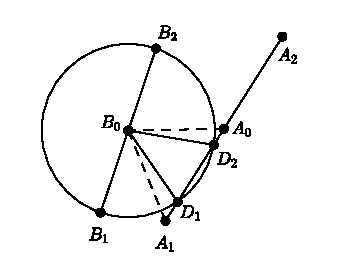
\includegraphics[width=0.35\linewidth]{lem8.eps}}
	\caption{Пояснение к лемме \ref{th:lem8}}
	\label{pic:lem8}
\end{figure}

\begin{lemma}
\label{th:lem9}
Если два моста $AA_1$ и $BB_1$ одной ТД пересекают ребро $PQ$ другой ТД, и концевая точка $P$ ребра попадает внутрь обеих окружностей влияния мостов, то разность углов $\angle APA_1$ и $\angle BPB_1$ не меньше $60^\circ$. 
\end{lemma}

\begin{proof}
С окружностью влияния моста $BB_1$ мост $AA_1$ имеет две точки пересечения $D_1$ и $D_2$ (рис. \ref{pic:lem9}).
Поскольку угол $\angle BPB_1$ лежит внутри $\angle APA_1$, имеем $\angle APA_1 = \angle BPB_1 + \angle APB + \angle A_1PB_1$.
Очевидно, что $\angle APB \ge \angle D_1PB \ge 0.5 \wideparen{D_1B}$ и $\angle A_1PB_1 \ge \angle D_2PB_1 \ge 0.5 \wideparen{D_2B_1}$. 
Тогда $\angle APB + \angle A_1PB_1 \ge 0.5(\wideparen{D_1B} + \wideparen{D_2B_1}) = 0.5(180^\circ - \wideparen{D_1D_2})$.
Но согласно лемме \ref{th:lem8} имеем $\wideparen{D_1D_2} \le 60^\circ$.
Поэтому $\angle APB + \angle A_1PB_1 \ge 0.5(180^\circ - 60^\circ) = 60^\circ$.
Следовательно, $\angle APA_1 \ge \angle BPB_1 + 60^\circ$, что и требовалось доказать.
\end{proof}

\begin{figure}[htb!]
	\center{\includegraphics[width=0.35\linewidth]{lem9.png}}
	\caption{Пояснение к лемме \ref{th:lem9}}
	\label{pic:lem9}
\end{figure}

\begin{lemma}
\label{th:lem10}
Если ребро ТД пересекает несколько мостов другой ТД, то концевая точка ребра может попасть внутрь окружностей влияния не более чем двух мостов.
\end{lemma}

\begin{proof}
Пусть ребро $PQ$ пересекает несколько мостов, и точка $P$ попадает внутрь окружностей влияния трех мостов $AA_1$, $BB_1$ и $CC_1$ (рис.\ref{pic:lem10}).
Тогда согласно лемме \ref{th:lem9} имеем: $\angle APA_1 \ge \angle BPB_1 + 60^\circ \ge \angle CPC_1 + 120^\circ$.
Но $\angle APA_1 \le 180^\circ$, и поэтому $CPC_1 \le 60^\circ$.
Поскольку угол $\angle CPC_1$ опирается на диаметр окружности влияния $CC_1$, то  точка $P$ лежит внутри этого круга.
Следовательно, он должен быть не менее $90^\circ$.
Полученное противоречие показывает, что точка $P$ не может оказаться внутри окружности влияния третьего моста $CC_1$, что и требовалось доказать. 
\end{proof}

\begin{figure}[htb!]
	\center{\includegraphics[width=0.35\linewidth]{lem10.png}}
	\caption{Пояснение к лемме \ref{th:lem10}}
	\label{pic:lem10}
\end{figure}

Теперь можно оценить количество мостов ТД, которые может разрушить ребро другой ТД при их объединении.

\begin{theorem}
\label{th:th1}
При объединении двух ТД каждое ребро пересекается не более чем с четырьмя мостами, которые оно разрушает. 
\end{theorem}

\begin{proof}
Непосредственно следует из леммы \ref{th:lem10}.
Поскольку разрушение моста ребром происходит лишь при попадании конца ребра внутрь окружности влияния моста,
а по лемме \ref{th:lem10} один конец ребра может попасть лишь в две такие окружности,
общее число разрушенных одним ребром мостов не превышает четырех.
\end{proof}

На основании теоремы \ref{th:th1} можно теперь оценить общее время поиска всех стартеров.
При локализации моста осуществляется анализ всех пересечений моста с ребрами объединенной триангуляции.
При этом сам мост является одноцветным ребром одной из исходных триангуляций,
а пересекаемые им ребра являются либо разноцветными, либо одноцветными, но противоположного цвета с мостом.
Если два отрезка пересекаются и каждый из них является ребром Делоне в своей триангуляции, то в объединенную триангуляцию один из них не должен входить. Это прямо следует из леммы \ref{th:lem1}.
Следовательно, либо мост разрушает ребро, либо ребро разрушает мост.
Те ребра, которые мост разрушает, имеют одно пересечение с одним мостом, так как к моменту анализа следующего моста эти ребра уже разрушены.
Те ребра, которые сами разрушают мост, могут разрушить не более четырех мостов каждое.
Следовательно, общее количество пересечений мостов с ребрами не может превысить пятикратное число ребер во всех триангуляциях, т.е. составляет $O(n)$. Таким образом, справедлива следующая теорема:

\begin{theorem}
\label{th:th2}
Вычислительная сложность алгоритма поиска всех стартеров составляет $O(n)$.
\end{theorem}

\subsection{Сложность построения разрезов и швов}
На этом шаге алгоритма разрушаются одноцветные ребра,
которые перестали удовлетворять условию Делоне в объединенной триангуляции,
и строятся разноцветные ребра.
Построение нового разноцветного ребра осуществляется на основе углового критерия (лемма \ref{th:lem1}) для пары конкурирующих ребер,
т.е. занимает фиксированное время $O(1)$.
Для каждого нового разноцветного ребра выполняется оценка корректности соседних с ним одноцветных ребер.
Такая проверка дважды запускает угловой критерий.
Если по результатам тестирования какое-то ребро уничтожается, то ставшее соседним другое одноцветное ребро вновь подвергается тесту.
Таким образом, время на удаление одного одноцветного ребра также оценивается как постоянное $O(1)$.

К общему времени стоит ещё добавить время включения нового ребра в триангуляцию.
При включении первого стежка, образуемого из стартера, может потребоваться полный перебор всех ребер, входящих в пучки двух инцидентных ему сайтов. Поэтому, общее время включения всех начальных ребер в пучки оценивается как $O(n)$.
А вот включение каждого очередного ребра уже не требует перебора ребер,
поскольку новое ребро устанавливается в пучок вслед за текущим анализируемым ребром.
Поэтому общее время на включение всех ребер есть $O(n)$.

Общее число построенных ребер не превосходит количество ребер в выходной триангуляции, то есть $O(n)$,
а общее число разрушенных ребер не превосходит общее число ребер в исходных триангуляциях --- тоже $O(n)$.
Таким образом, с учетом теоремы \ref{th:th2} нами доказана теорема:

\begin{theorem}
\label{th:th3}
Предложенный алгоритм объединяет две неразделенные триангуляции Делоне за время $O(n)$.
\end{theorem}

Очевидно, что размер памяти, используемой при работе алгоритма, составляет также   $O(n)$.

\section{Заключение}
В данной статье был предложен вычислительно эффективный алгоритм объединения двух перекрывающихся триангуляций Делоне.
Оценка вычислительной сложности алгоритма была доказана, предложенный подход был теоретически обоснован.
Предложенный метод позволяет эффективно производить сравнение $3D$ поверхностей, при этом построение двух исходных ТД и МОД производится один раз, и относится к этапу предобработки, объединение триангуляций на каждом шаге подгонки поверхностей будет производиться за $O(n)$.
Таким образом, общая оценка вычислительной сложности алгоритма равна $O(n\log n) + O(mn)$, где $n$ --- общее число точек двух исходных триангуляций, $m$ --- число итераций.

Работа выполнена при поддержке Российского Фонда фундаментальных исследований (РФФИ), проект 14-01-00716-a.

\newpage
\bibliographystyle{utf8gost705u}
\bibliography{ru_article}{}

\end{document}